\documentclass[../main]{subfiles}
\begin{document}
    \setcounter{secnumdepth}{2}
    \chapter{序論}
        \section{背景}
        近年,商業施設での掃除や屋外での宅配など,多くの場所で自律移動ロボットが活用されている.それらのロボットが安全に自律移動するには,
        自己位置推定や経路計画といった様々な機能が必要となる.
        ロボットの自律移動によく用いられる地図として,メトリックマップと呼ばれるものがある.
        
        
        一方,人はそのような詳細な地図がなくても,「2つ目の信号で右」のような簡単な情報により目的地まで移動することができる.
        そこで,そのような人の移動する能力をロボットの自律移動に応用する手法が研究されている.例えば,島田らは人の道案内に注目し,
        トポロジカルマップとシナリオによるナビゲーション手法を提案した.この研究では,人が目的地まで移動する際に必要としている情報をアンケートにより取得し,
        得られた情報からナビゲーションに用いるトポロジカルマップと呼ばれる地図と,シナリオと呼ばれる人の道案内を言葉にしたものの形式を決定し,
        人の道案内のようにロボットを目的地まで移動させるナビゲーションの手法を提案した.また,提案したナビゲーション手法の有効性を実機を用いた実験により検証した.
        実験の結果,通路の認識が正しく行われた場合は,提案したナビゲーション手法により目的地に到達できるが,
        誤認識が起きた場合はロボットが経路から外れ,ナビゲーションに失敗してしまうということが報告されている.
        先行研究では,通路の認識にはLiDARを使用しており,通路の誤認識は,開いているドアや隙間にLiDARが反応したことが原因であると述べられている.
        ここで,通路の認識にカメラ画像を用いることで,誤認識を解消し,ナビゲーション途中に経路から外れるという問題を解決できるのではないかと考えた.

        \newpage

        \section{目的}
        本研究は,全天球カメラ画像に基づく通路認識の手法を提案する.そして,先行研究により提案された,実ロボットを用いた
        トポロジカルマップとシナリオに基づくナビゲーションに対し,認識した通路の特徴情報を適用することで本手法の有効性を検証する.
        検証の際は,本研究と先行研究のナビゲーション結果に着目し,その成功回数を比較することとする.


        また,本研究では\fref{figure::image_exp}に示すような,全天球カメラの標準的なフォーマットである正距円筒図法という形式で画像を扱う.

        \begin{figure}[H]
            \centering
            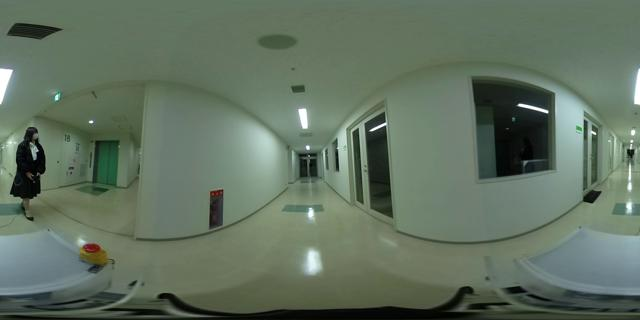
\includegraphics[width=10cm]{../images/18F_aisle_exp.jpg}
            \caption{Example of spherical camera image of equirectangular projection.}
            \label{figure::image_exp}
        \end{figure}
        
        \newpage

        \section{関連研究}
        \section{本論文の構成}
        本論文ではまず,第1章で研究背景,目的,関連研究について述べた.第2章では,本研究で用いる要素技術について述べる.また,第3章では提案した手法について述べ,
        第4章では提案した手法の有効性の検証を行う.また,第5章では4章で行なった実験の結果をまとめ,考察を行う.最後に,第6章で本研究のまとめを行う.
\end{document}